
\title{The Name of the Title Is Hope} % \title[short title]{Full title}

\begin{abstract}
  A clear and well-documented \LaTeX\ document is presented as an article formatted for publication by ACM in a conference proceedings or journal publication. Based on the ``acmart'' document class, this article presents and explains many of the common variations, as well as many of the formatting elements an author may use in the preparation of the documentation of their work.
\end{abstract}

%% Keywords. The author(s) should pick words that accurately describe the work being presented. Separate the keywords with commas.
\keywords{Do, Not, Us, This, Code, Put, the, Correct, Terms, for, Your, Paper}

%% A "teaser" image appears between the author and affiliation information and the body of the document, and typically spans the page.
\begin{teaserfigure}
  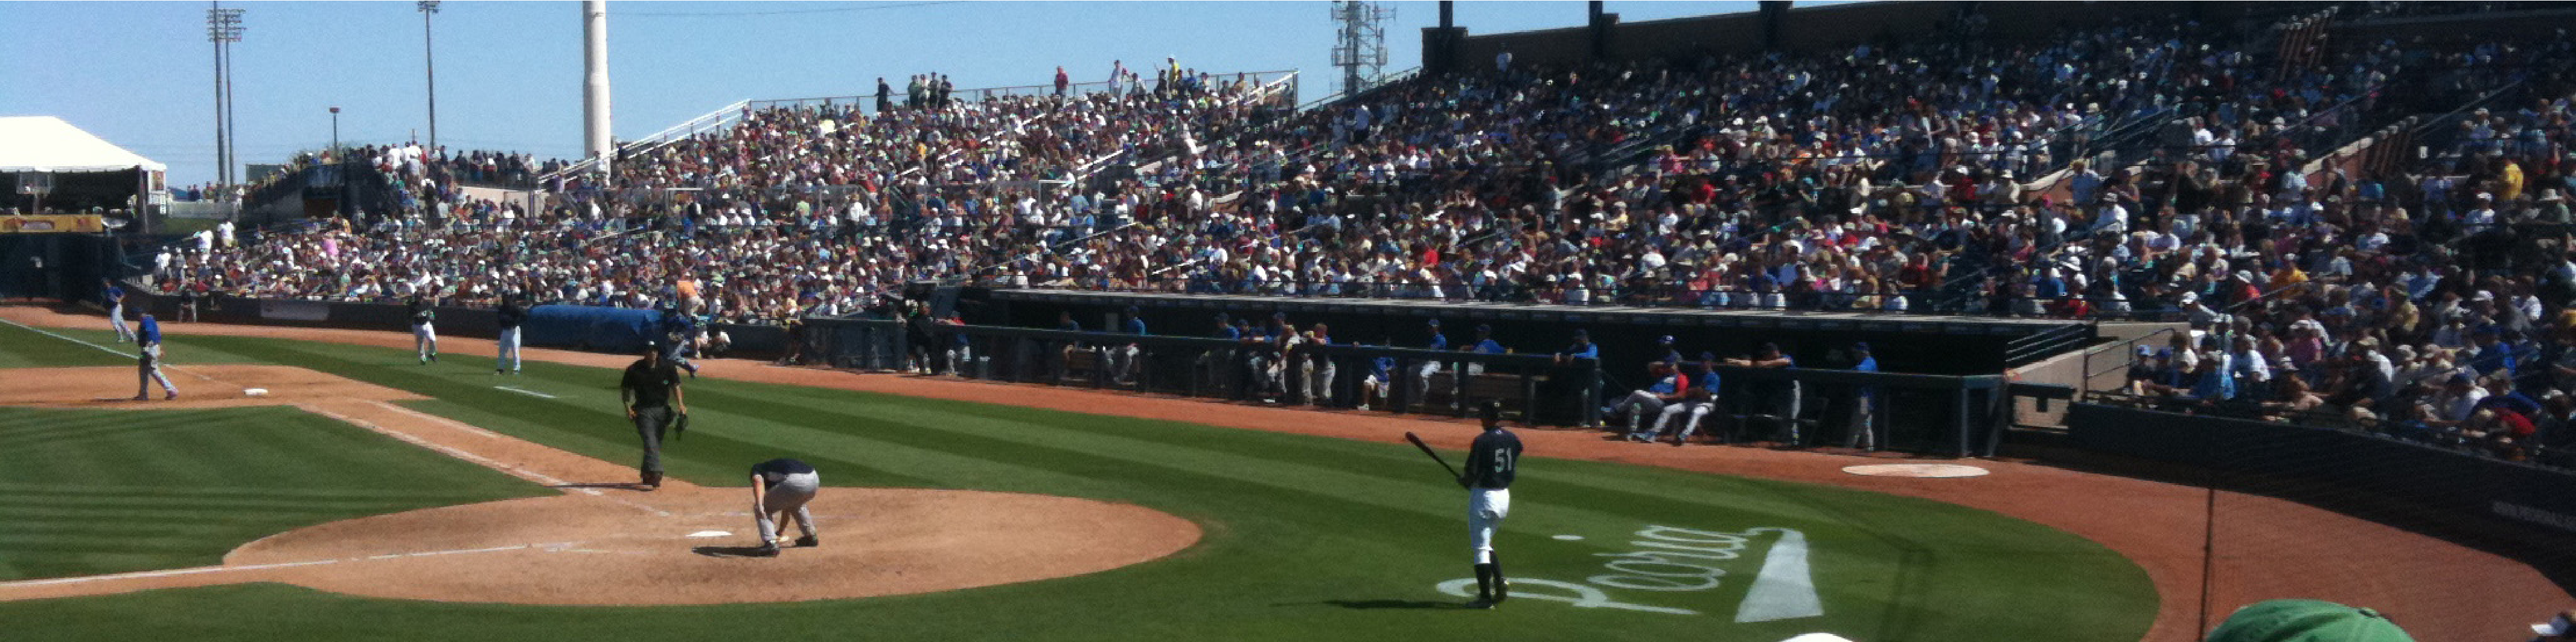
\includegraphics[width=\textwidth]{sampleteaser}
  \caption{Seattle Mariners at Spring Training, 2010.}
  \Description{Enjoying the baseball game from the third-base seats. Ichiro Suzuki preparing to bat.}
  \label{fig:teaser}
\end{teaserfigure}

\received{20 February 2007}
\received[revised]{12 March 2009}
\received[accepted]{5 June 2009}

%% This command processes the author and affiliation and title information and builds the first part of the formatted document.
\maketitle

